\chapter{Odczytywanie losowego wyniku z kości}\label{ch:odczytywanie-losowego-wyniku-z-kosci}

Kolejnym krokiem przetwarzania -- po wykonaniu rzutu i zdjęcia -- jest odczyt wylosowanej wartości z kości.
Jak pokazano na rys.~\ref{fig:schemat_workflow},
najpierw zdjęcie musi zostać poddane odpowiedniemu przetwarzaniu, które zostało opisane w tym rozdziale.

\begin{figure}[H]
    \centering
    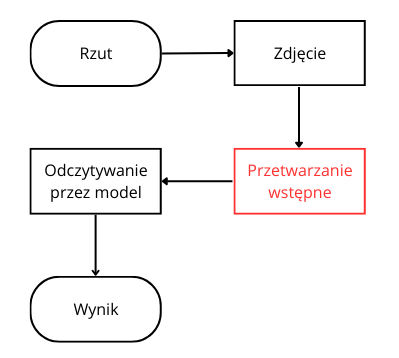
\includegraphics[width=0.5\linewidth]{chapters/04-czytanie/figures/schemat.png}
    \caption{Schemat pracy robota}
    \label{fig:schemat_workflow}
\end{figure}

\section{Przetwarzanie wstępne obrazów}\label{sec:preprocessing}

W niniejszym rozdziale omówiono proces przetwarzania wstępnego obrazów kości,
który przekształca dane pochodzące z fizycznego komponentu robota (kamery dostarczającej zdjęcia kości) na dane wejściowe dla modelu sztucznej inteligencji.
Przez dane wejściowe dla modelu SI rozumie się tutaj odpowiednio sformatowane obrazy, a więc takie w skali szarości,
o rozmiarach $64\times64$ piksele, zawierające jedynie kość wyciętą ze zdjęcia (nie zawierające w tle całego kubka).

\subsection{Algorytm}\label{subsec:algorytm}

\begin{enumerate}
    \item Wczytanie obrazu wejściowego.
    \item Odnalezienie kości za pomocą maski na komponencie nasycenia.
    \item Stworzenie i wycięcie ramki ograniczającej (ang. \textit{bounding box}) wokół maski.
    \item Przeskalowanie do odpowiedniego rozmiaru.
    \item Konwersja do skali szarości.
    \item Zapisanie gotowego obrazu.
\end{enumerate}

Na rys.~\ref{fig:preproc_steps} przedstawiono przykładowe zdjęcie surowe~\ref{fig:step1}
oraz kolejne etapy przetwarzania, aż do finalnego etapu~\ref{fig:step5}.

\begin{figure}[H]
    \centering
    \begin{subfigure}[t]{0.32\linewidth}
        \centering
        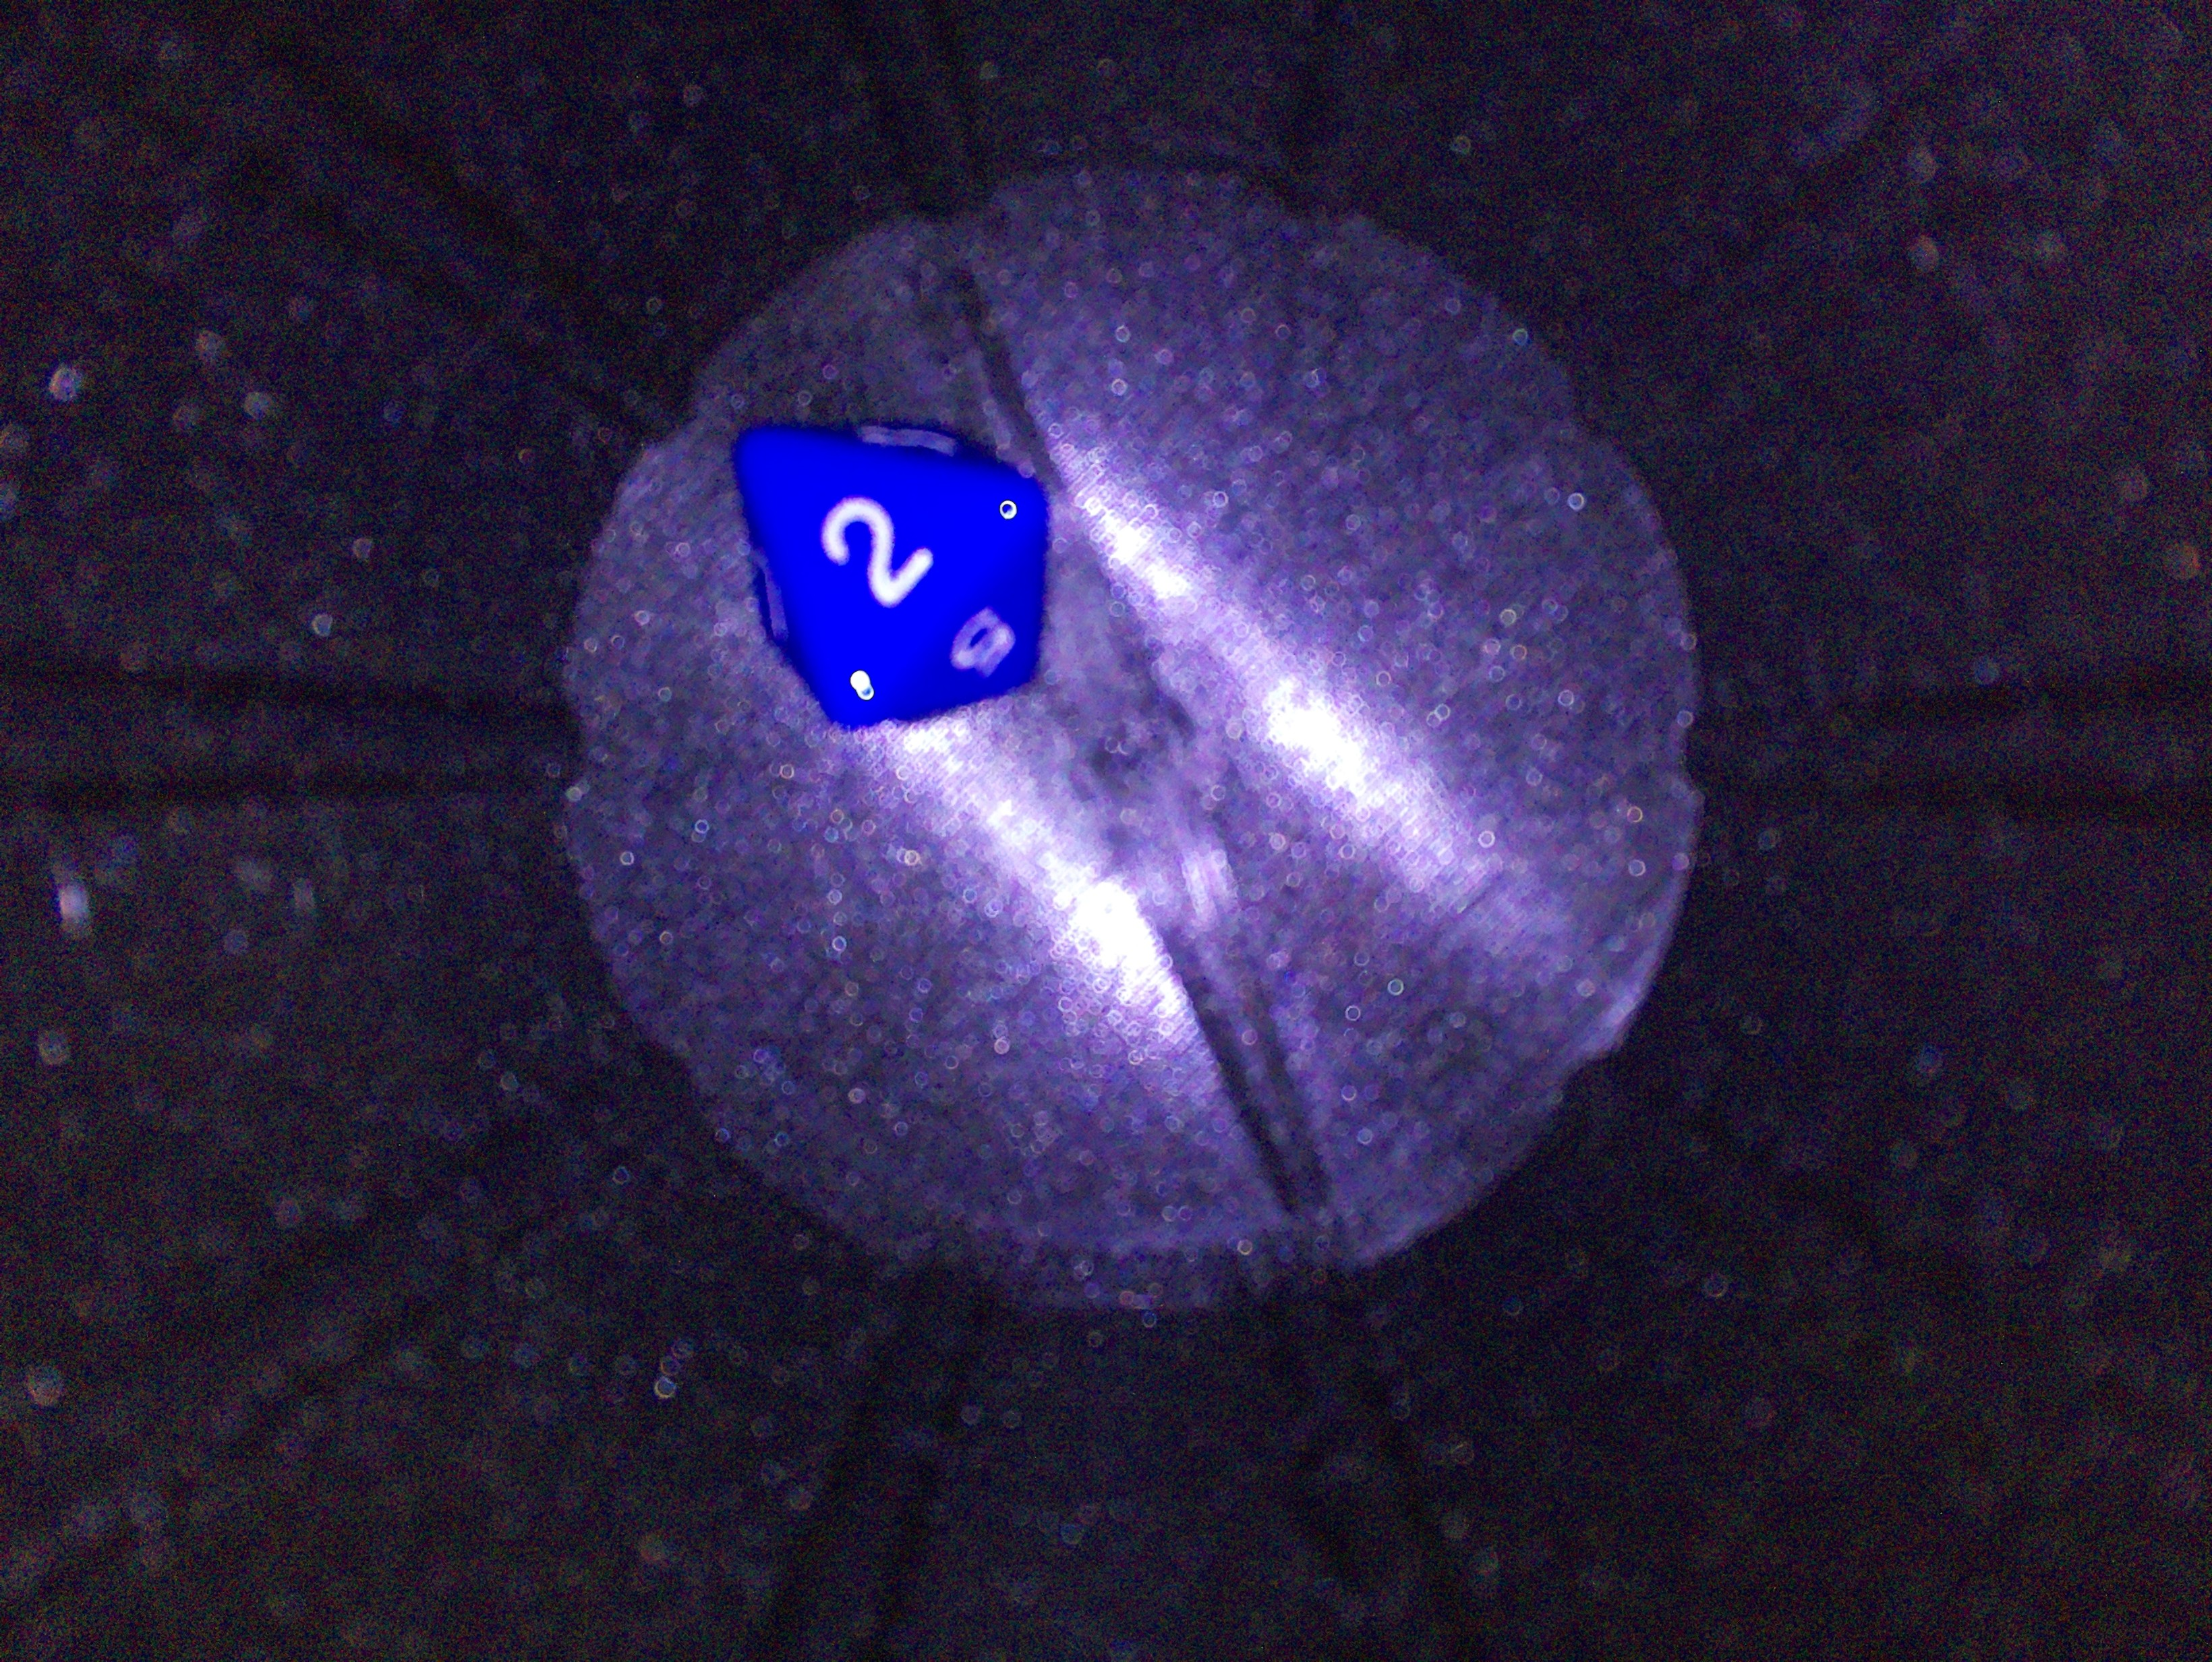
\includegraphics[height=4cm]{chapters/04-czytanie/figures/2_1}
        \caption{Etap 1: Surowe zdjęcie.}
        \label{fig:step1}
    \end{subfigure}
    \hspace{-0.5em}
    \begin{subfigure}[t]{0.32\linewidth}
        \centering
        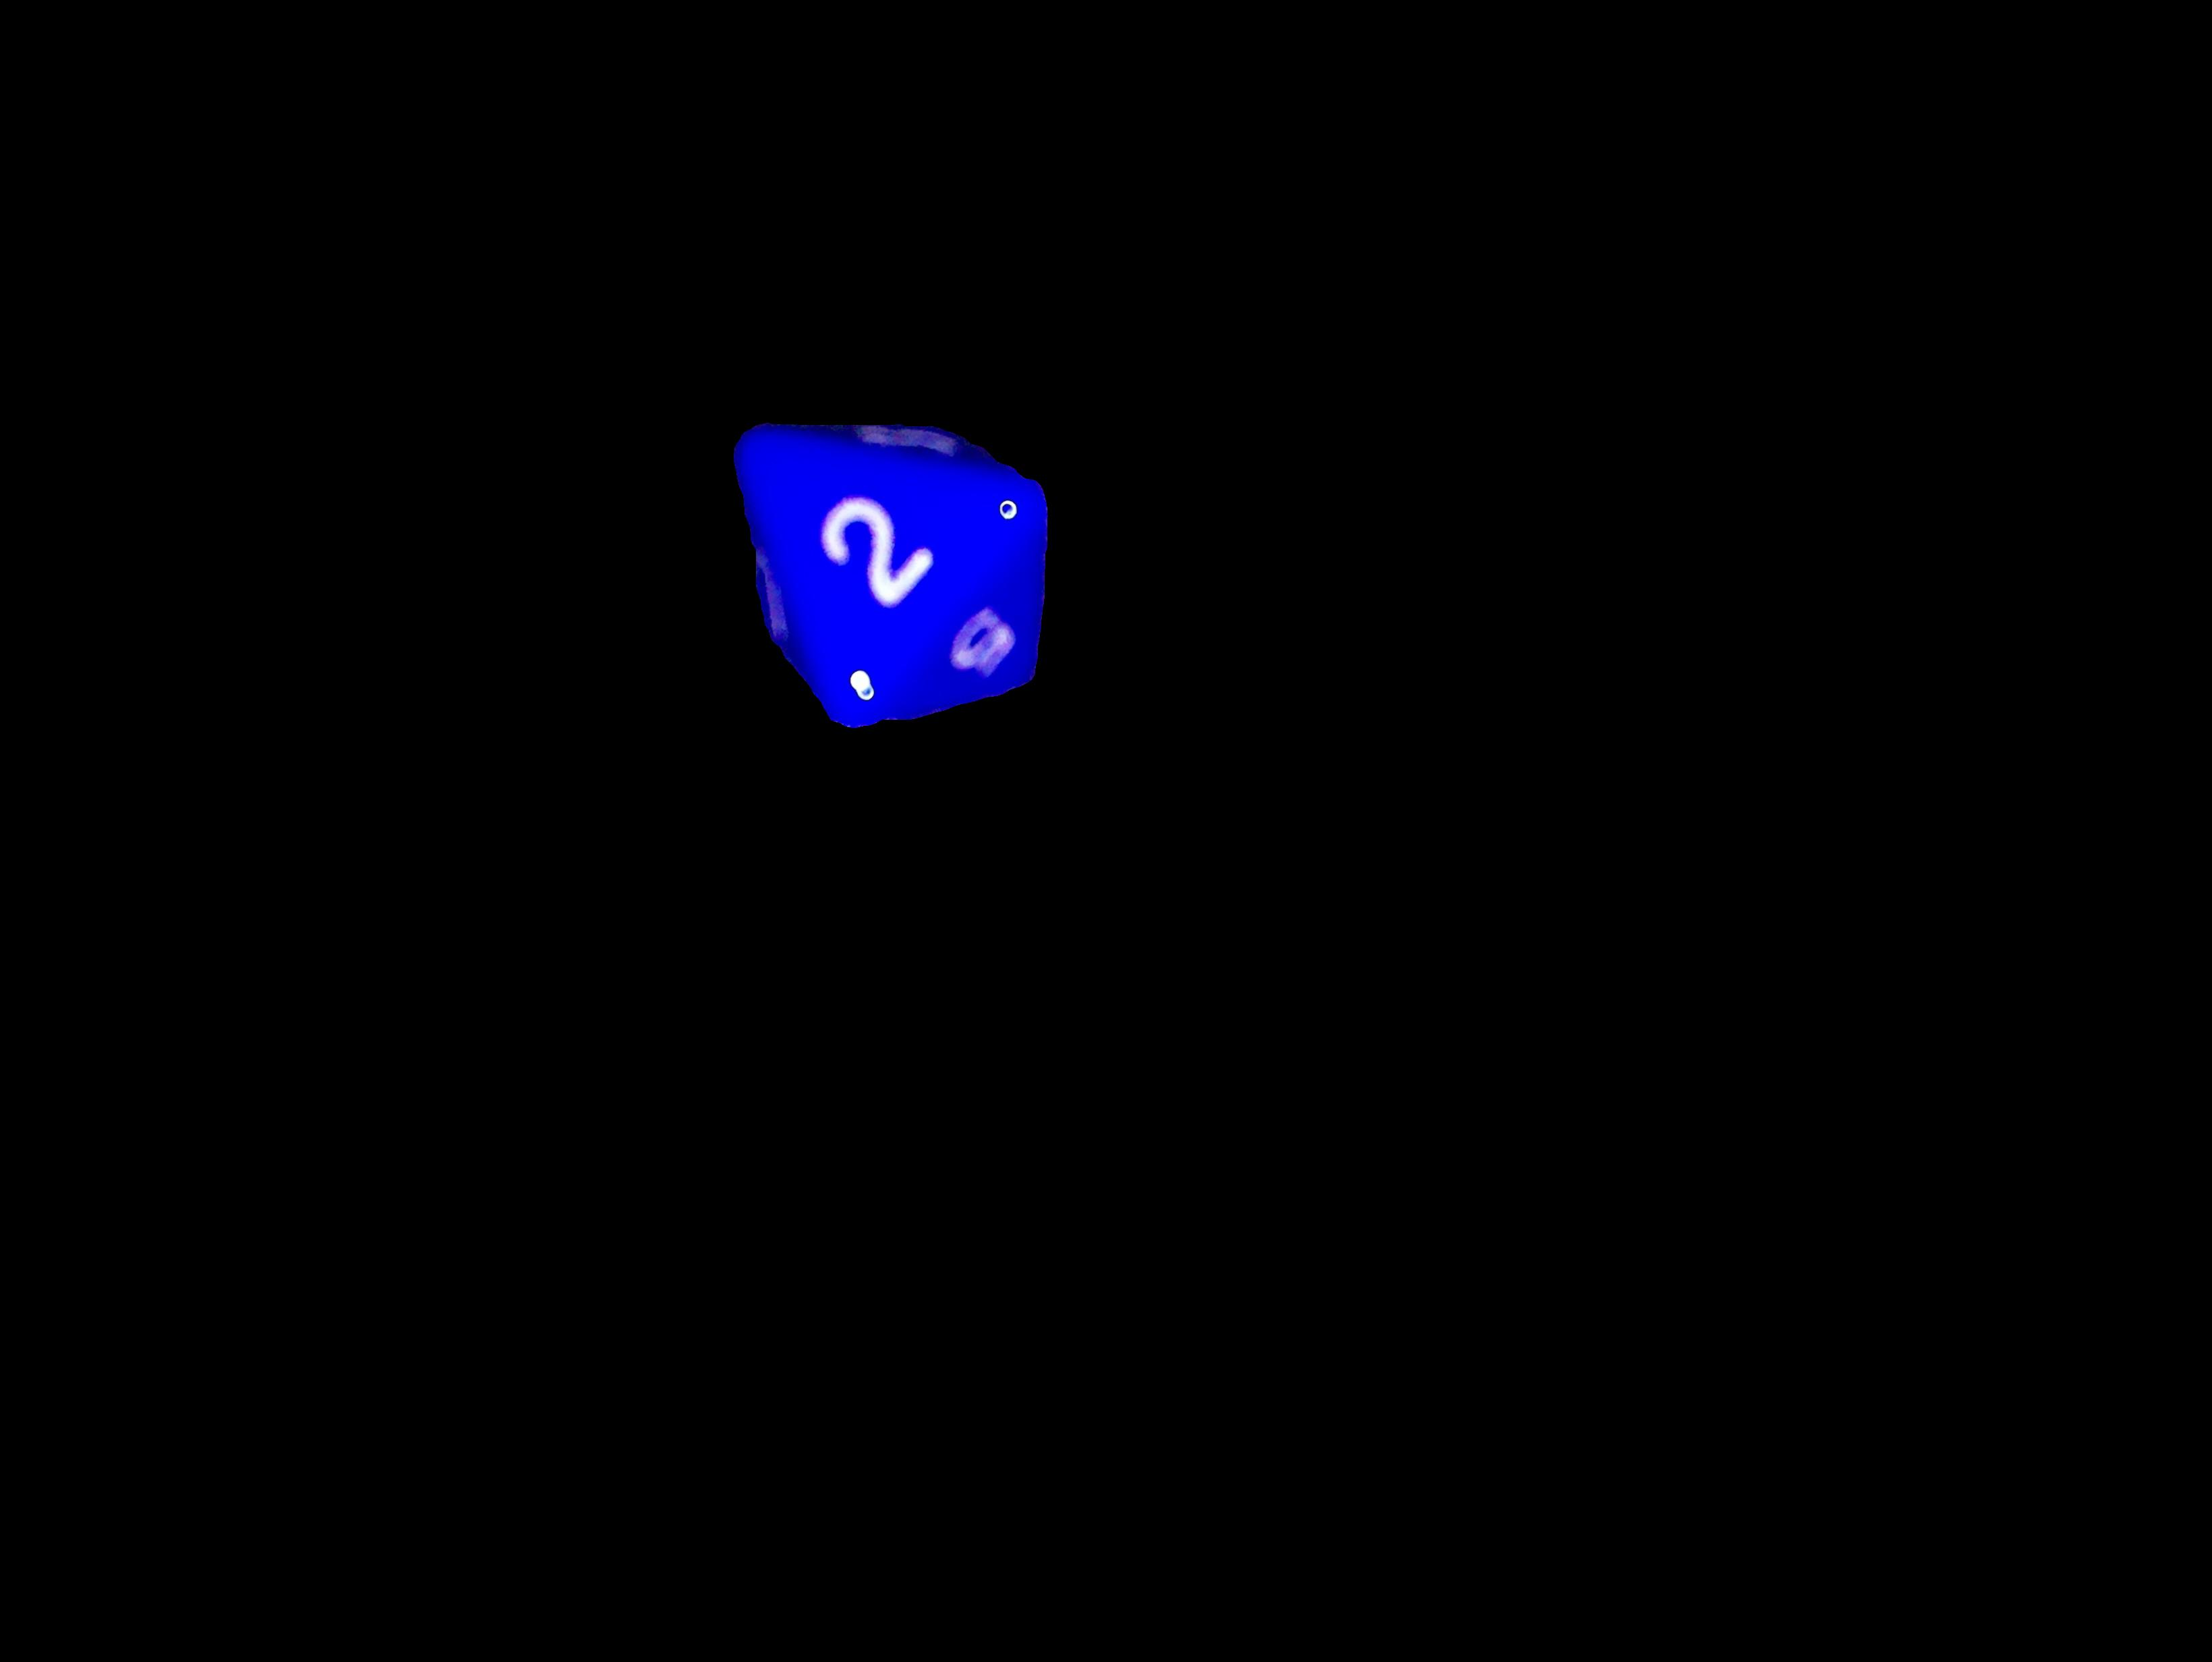
\includegraphics[height=4cm]{chapters/04-czytanie/figures/2_2}
        \caption{Etap 2: Nałożenie maski}
        \label{fig:step2}
    \end{subfigure}
    \hspace{-0.5em}
    \begin{subfigure}[t]{0.32\linewidth}
        \centering
        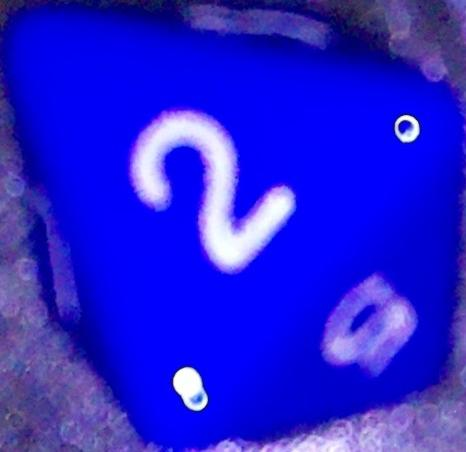
\includegraphics[height=4cm]{chapters/04-czytanie/figures/2_3}
        \caption{Etap 3: Wycięcie obszaru zainteresowania}
        \label{fig:step3}
    \end{subfigure}

    \vspace{0.3cm}

    \begin{subfigure}[t]{0.45\linewidth}
        \centering
        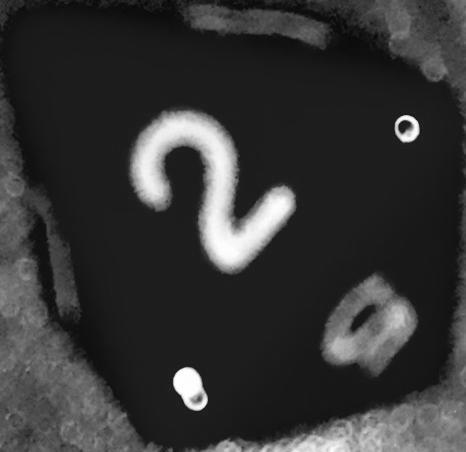
\includegraphics[height=4cm]{chapters/04-czytanie/figures/2_4}
        \caption{Etap 4: Skala szarości}
        \label{fig:step4}
    \end{subfigure}
    \hspace{0.5em}
    \begin{subfigure}[t]{0.45\linewidth}
        \centering
        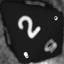
\includegraphics[height=4cm]{chapters/04-czytanie/figures/2_5}
        \caption{Etap 5: Wynik końcowy.}
        \label{fig:step5}
    \end{subfigure}

    \caption{Kolejne etapy przetwarzania obrazu. Wszystkie obrazy mają równą wysokość.}
    \label{fig:preproc_steps}
\end{figure}


Przedstawiony algorytm został zaimplementowany w języku Python, a jego zadaniem jest identyfikacja,
wycięcie i przeskalowanie obszarów zawierających obiekty zainteresowania na zdjęciach.

Zdjęcia w formacie JPEG są wczytywane za pomocą modułu Pillow~\cite{pillow_docs},
który umożliwia konwersję obrazów do przestrzeni barw RGB, zapewniając jednolitość formatów danych wejściowych.
Następnie obrazy są przekształcane do przestrzeni barw HSV,
co pozwala oddzielić komponenty odpowiadające za barwę (H), nasycenie (S) oraz jasność (V).

Komponent nasycenia (S) jest wygładzany za pomocą filtru Gaussa~\cite{gaussian_filter},
również dostępnego w ramach tego samego modułu,
co redukuje szumy i pozwala na bardziej precyzyjną analizę.
Wykorzystano parametry filtru z maską o wymiarach $5 \times 5$ pikseli oraz odchyleniem standardowym równym 1.
Takie ustawienia zapewniają balans między wygładzeniem a zachowaniem szczegółów obrazu.

Na podstawie wygładzonego komponentu nasycenia za pomocą progowania tworzona jest maska binarna,
która identyfikuje obszary o wysokim nasyceniu, odpowiadające obiektom zainteresowania (kości).
Próg został dobrany eksperymentalnie, kończąc na wartości 224,
tak aby w kontrolowanym środowisku (opisanym w poprzednim rozdziale) maska obejmowała obszar zainteresowania,
ale nie obejmowała tła (czarnego kubka).
Korzysta to z faktu, że kubek wykonany jest z materiału o niskim nasyceniu,
a używana kość ma jednolity, jasny kolor, a więc i wysokie nasycenie.

W celu usunięcia niewielkich luk w masce binarnej stosowana jest operacja zamknięcia morfologicznego~\cite{morphological_closure}.
Operacja ta ujednolica maskę, co jest szczególnie istotne w przypadku obiektów o niejednorodnej strukturze nasycenia,
gdzie maska mogłaby zawierać rozłączne fragmenty obiektu.

Po zastosowaniu zamknięcia morfologicznego maska jest analizowana w celu
zlokalizowania największego konturu obejmującego obszar zainteresowania.
W tym celu wykorzystano funkcje biblioteki OpenCV~\cite{opencv_docs},
które umożliwiają zarówno zastosowanie domknięcia morfologicznego, jak i wykrycie konturu, i obliczenie otaczającego go prostokąta.
Rozmiar prostokąta jest dynamicznie dopasowywany do obszaru maski.
%Domknięcie morfologiczne i zamknięcie morfologiczne to dokładnie to samo.

Na tej podstawie oryginalny obraz jest kadrowany w kształt prostokąta wokół obszaru zainteresowania,
a następnie przeskalowywany do wymiarów $64 \times 64$ pikseli.
Ostatecznie obraz jest konwertowany do skali szarości, co zmniejsza wymiarowość danych
i pozwala sieci neuronowej skupić się na strukturze obrazu.
Konwersja do skali szarości dodatkowo minimalizuje negatywny wpływ odblasków,
powstających gdy kość odbija światło wprost do kamery, co poprawia niezawodność analizy.


\subsection{Zidentyfikowane trudności i ich rozwiązania}\label{subsec:zidentyfikowane-trudnosci-i-ich-rozwiazania}

Wspomniane wcześniej odblaski znacznie pogarszają skuteczność odczytywania wyniku z kości.
Jednak zastosowanie skali szarości pozwoliło w znacznym stopniu pozbyć się tego problemu,
uwidaczniając widoczną na kości cyfrę, co pokazuje rys.~\ref{fig:blaskcombined}.

Dzięki zastosowaniu skali szarości łatwiej jest oddzielić jasne punkty, będące wynikiem odblasku światła diody od ściany kości,
od nieco ciemniejszych, lecz wciąż jasnych punktów oznaczających cyfrę na kości.

\begin{figure}[H]
    \centering
    \begin{subfigure}[t]{0.45\linewidth}
        \centering
        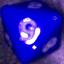
\includegraphics[width=\linewidth]{chapters/04-czytanie/figures/blask_raw}
        \caption{Odblask na przeskalowanym zdjęciu.}
        \label{fig:blaskraw}
    \end{subfigure}
    \hfill
    \begin{subfigure}[t]{0.45\linewidth}
        \centering
        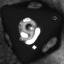
\includegraphics[width=\linewidth]{chapters/04-czytanie/figures/blask_proc}
        \caption{Odblask po zmianie na skalę szarości.}
        \label{fig:blaskproc}
    \end{subfigure}
    \caption{Porównanie odblasku przed i po przetworzeniu.}
    \label{fig:blaskcombined}
\end{figure}


Inną trudnością, która objawiała się w początkowych fazach pracy, były zupełnie czarne obrazy, ale
problem ten wynikał z usterki zastosowanej diody i został zażegnany poprzez fizyczną wymianę oświetlenia.
Obecnie taki problem jest wykrywany oraz zgłaszany jest wyjątek oznaczający potrzebę naprawy usterki oświetlenia.

Nie był to jedyny problem powodowany przede wszystkim częścią sprzętową -- drugim takim było zatrzymanie śmigła w miejscu,
przez co do ewaluacji przez model kilkukrotnie trafiało identyczne lub niemal identyczne zdjęcie.
To również zostało rozwiązane fizycznie, poprzez dodanie metalowej podkładki pod śmigłem,
ale mimo zażegnania problemu w taki sposób, zapewniono również obsługę wyjątku, który nadarzy się, gdy wielokrotnie zostanie odczytana identyczna wartość.
W związku z ryzykiem fałszywego rozpoznania zatarcia śmigła przez losowo wypadającą wielokrotnie identyczną wartość, ustawiono próg wykrywania takiej sytuacji i zgłaszania wyjątku na 13 identycznych odczytów z rzędu.
Statystyczna szansa na takie zdarzenie przy prawidłowej pracy maszyny wynosi
$\frac{1}{8^{12}} \approx 1{,}455 \cdot 10^{-11}$

Kolejną, znacznie częściej spotykaną trudnością w obecnej architekturze urządzenia są niejednoznaczne wyniki,
a więc moment, gdy kość zatrzyma się w pozycji, w której widać więcej niż jedną ściankę.
Najczęściej jest to spowodowane tym, że kość zatrzymała się na śmigle napędowym,
przez co wynik może być niejednoznaczny, co pokazano na rys.~\ref{fig:smiglocombined}.

\begin{figure}[h]
    \centering
    \begin{subfigure}[t]{0.45\linewidth}
        \centering
        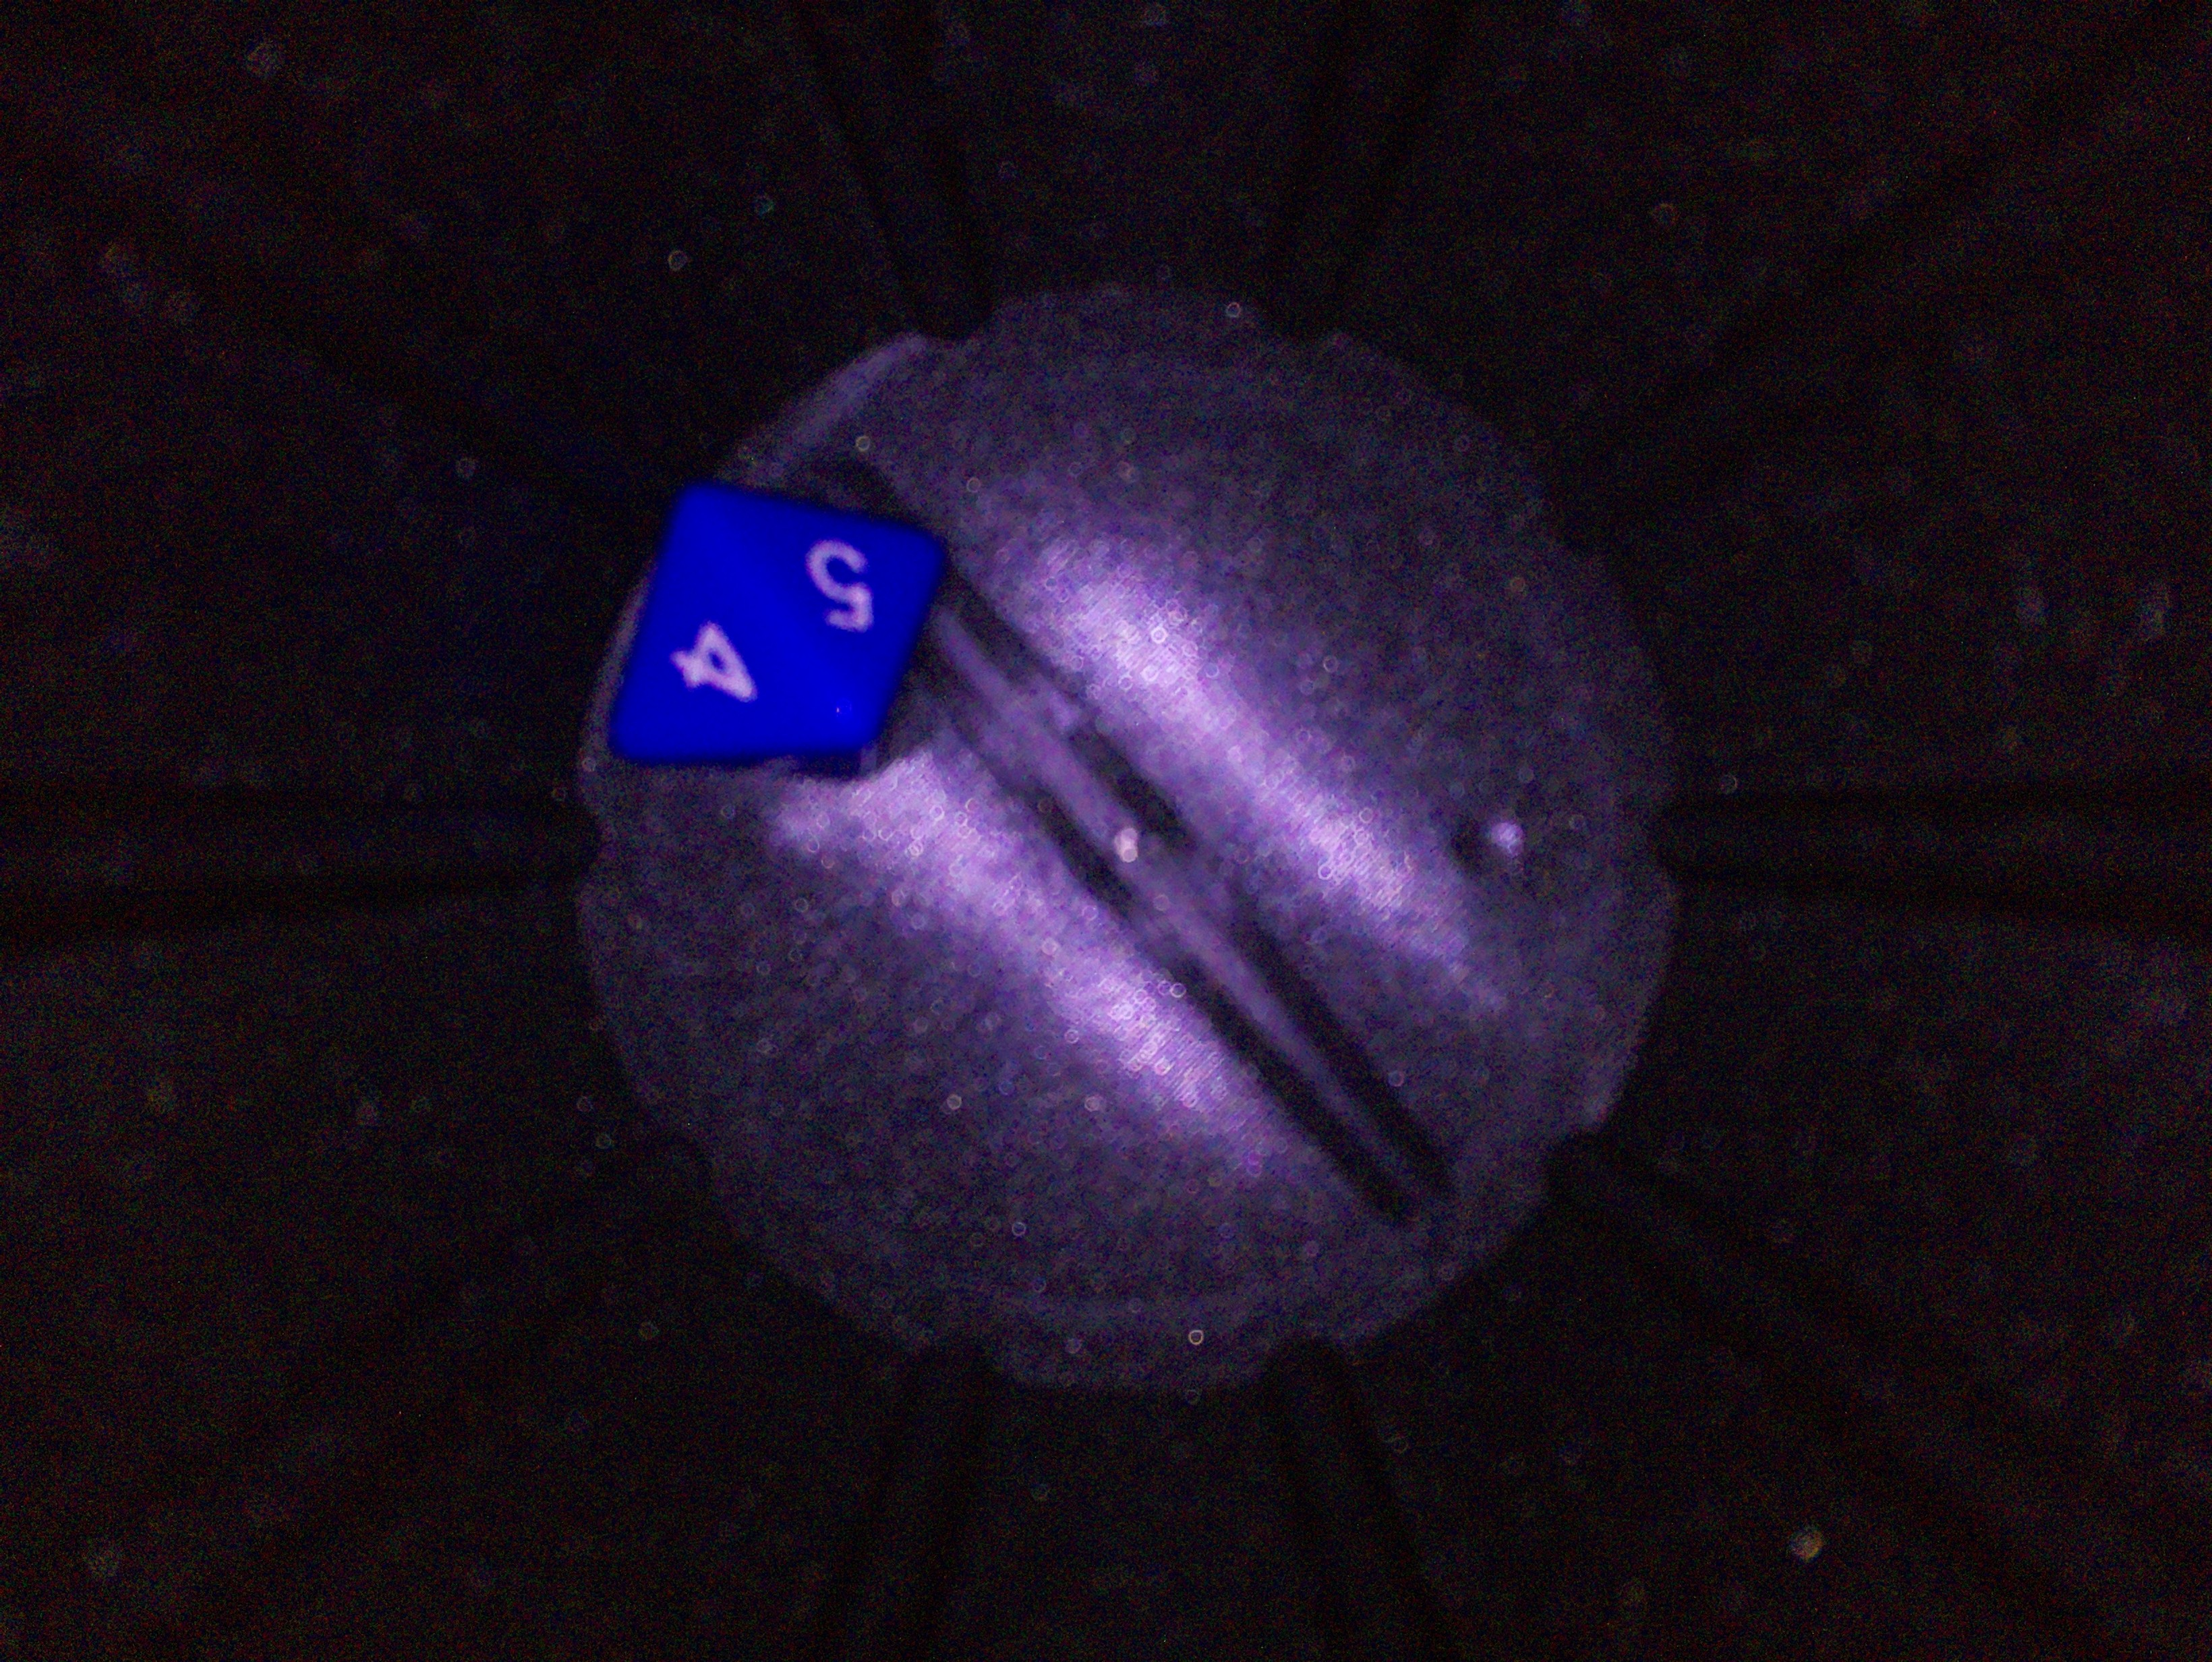
\includegraphics[width=\linewidth]{chapters/04-czytanie/figures/niepewne}
        \caption{Kość zatrzymana na śmigle (ujęcie 1).}
        \label{fig:niepewne}
    \end{subfigure}
    \hfill
    \begin{subfigure}[t]{0.45\linewidth}
        \centering
        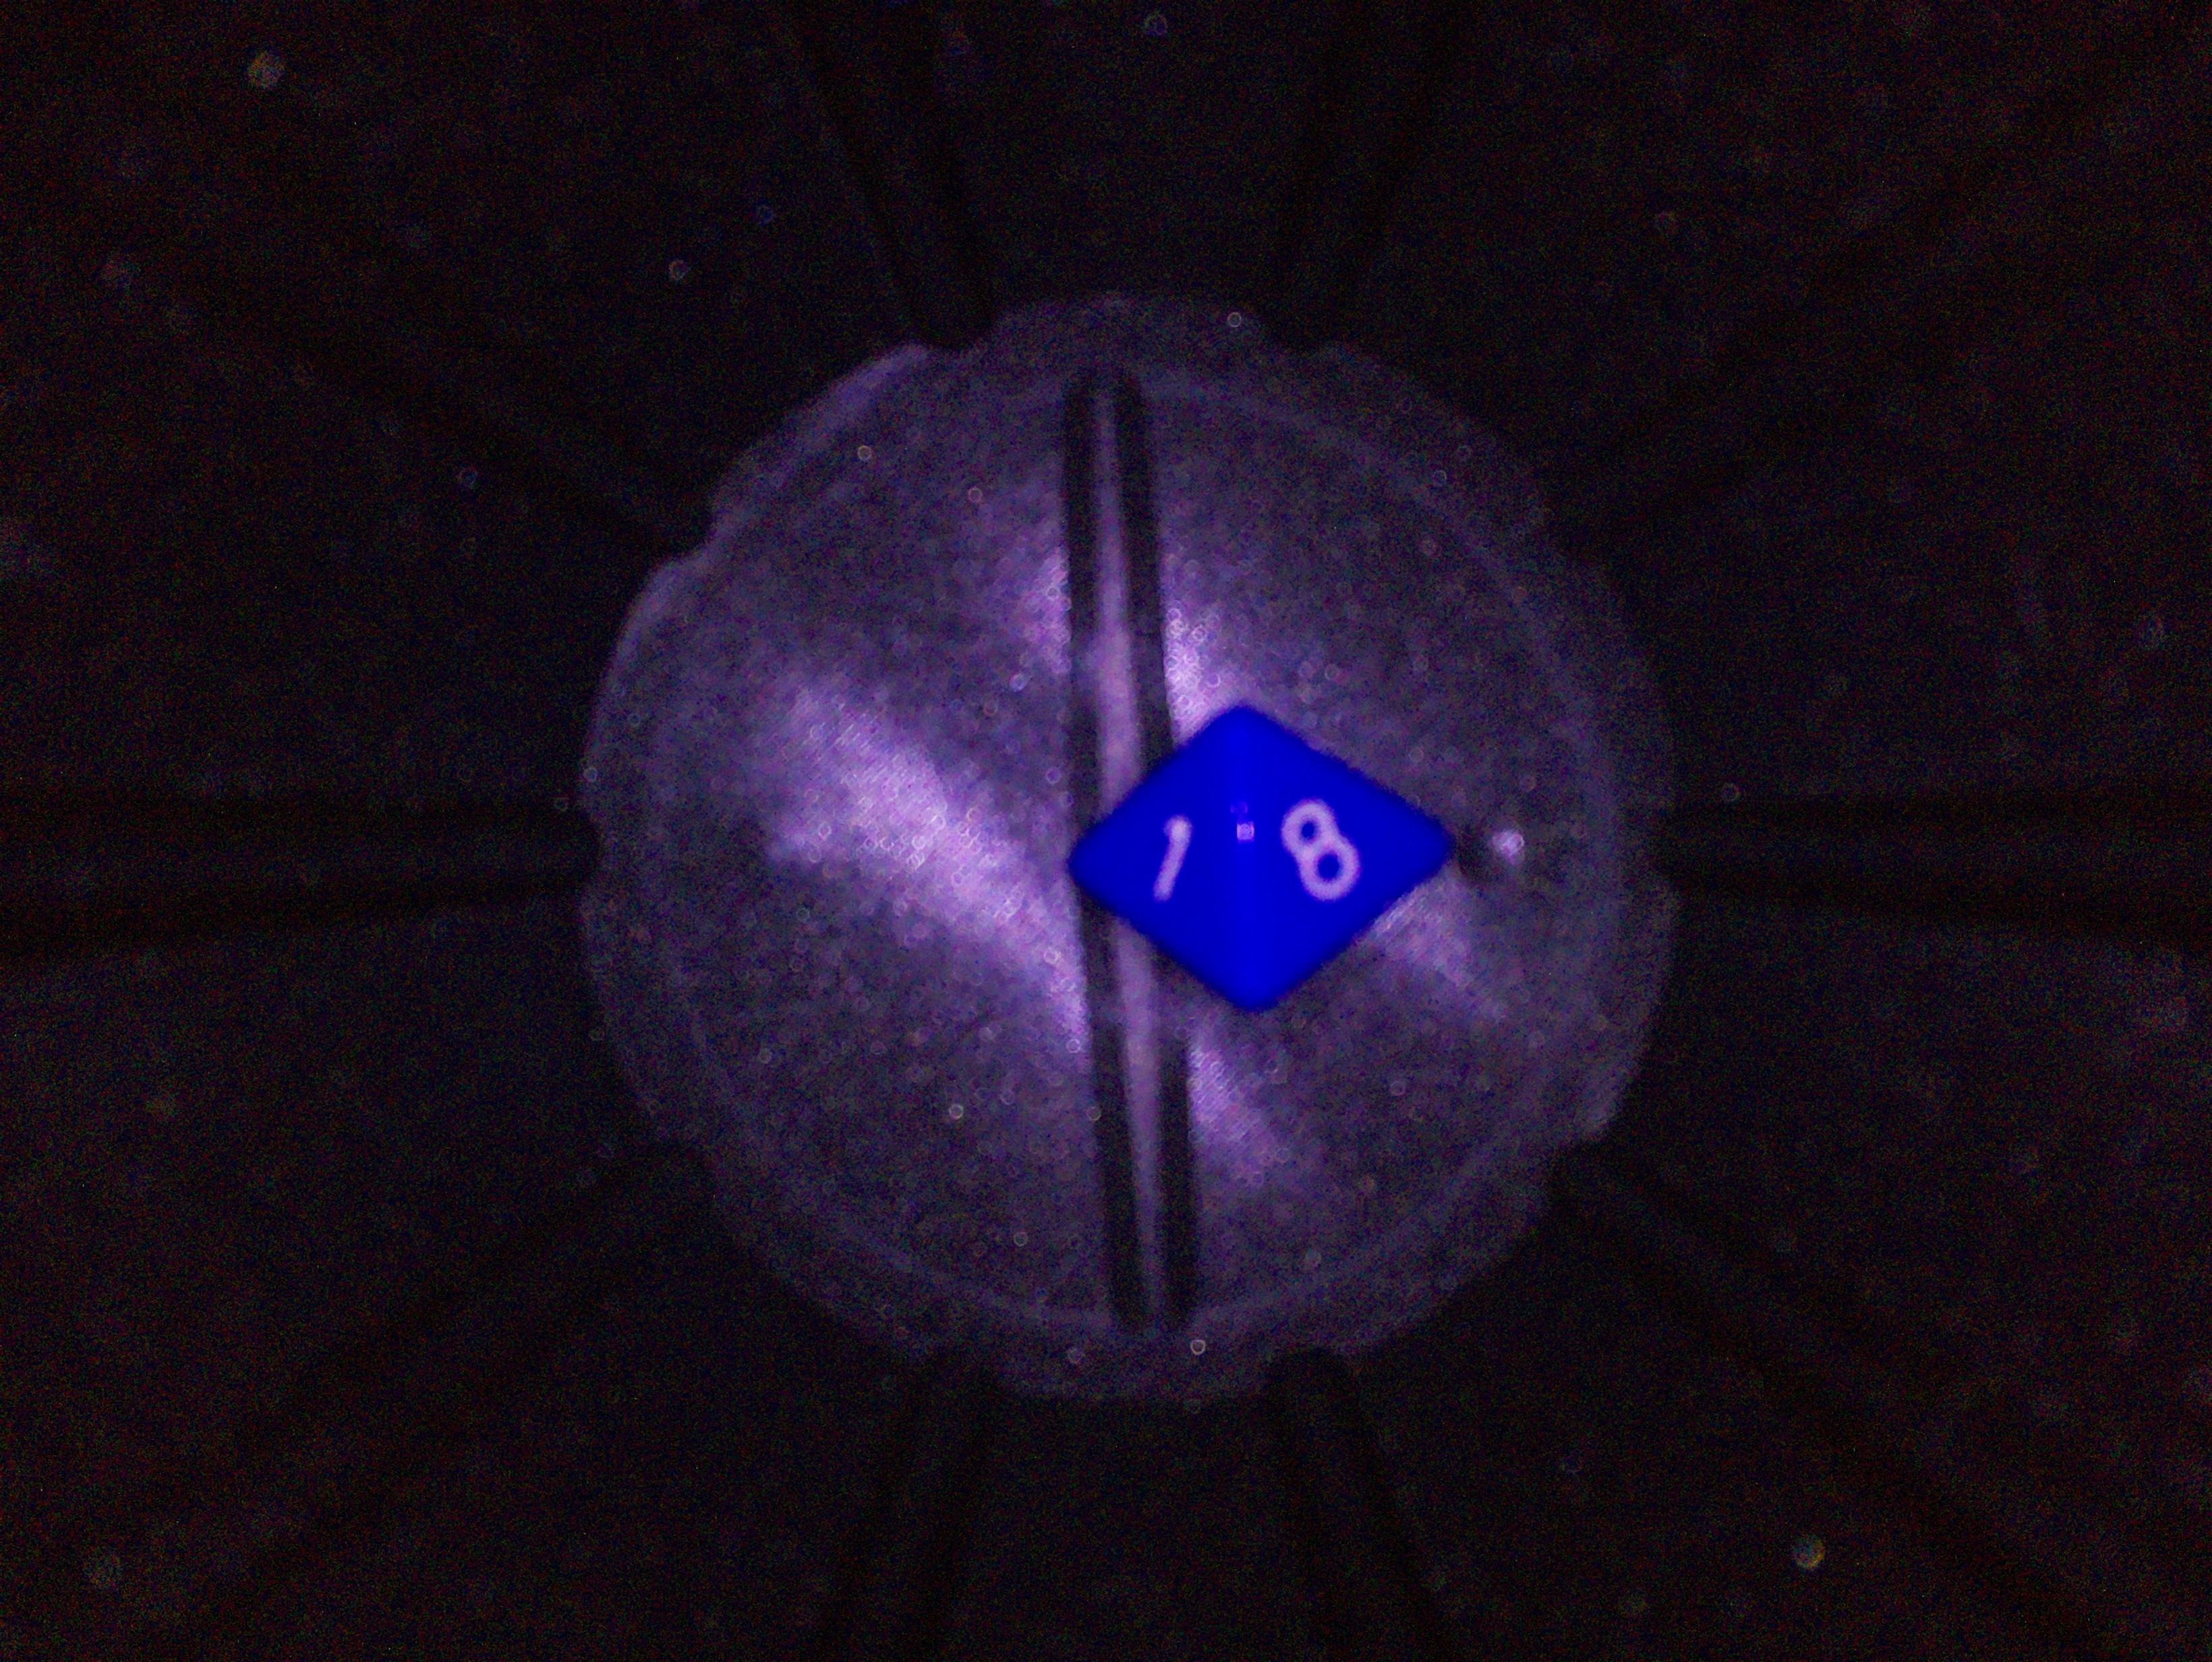
\includegraphics[width=\linewidth]{chapters/04-czytanie/figures/smiglo}
        \caption{Kość zatrzymana na śmigle (ujęcie 2).}
        \label{fig:smiglo}
    \end{subfigure}
    \caption{Porównanie dwóch ujęć kości zatrzymanej na śmigle.}
    \label{fig:smiglocombined}
\end{figure}


Rozwiązaniem tego problemu jest model dokonujący klasyfikacji wyniku rzutu, który odczytuje ze zdjęcia tylko jeden, najbardziej prawdopodobny wynik i wybiera ten,
który jest bardziej widoczny, ponieważ podczas uczenia model miał do czynienia z takimi niejednoznacznymi sytuacjami,
które zostały ręcznie oznaczone właśnie na potrzeby treningu modelu.

Zdarzają się również rzadkie przypadki, w których kość wyląduje równo na śmigle.
Jednakże w takim wypadku wynik jest idealnie czytelny,
identycznie jak gdy kość lądowała normalnie na podstawce kubka, więc nie jest to problemem.
%Wtedy problem z lądowaniem na śmigle nie istnieje,
%gdyż nie przeszkadza to w tym, że kość i tak zostanie podbita przy następnym obrocie śmigła.
Ostatnim rodzajem problemu, jaki został napotkany, był przypadek, w którym kość nie skończyła jeszcze swojej fazy lotu
lub wpadła w bardzo długie wirowanie -- efektywnie uniemożliwiając odczytanie wyniku.
Przykłady zarejestrowanych przypadków wystąpienia tego problemu przestawiono na rys~\ref{fig:wircombined}.

\begin{figure}[h]
    \centering
    \begin{subfigure}[t]{0.45\linewidth}
        \centering
        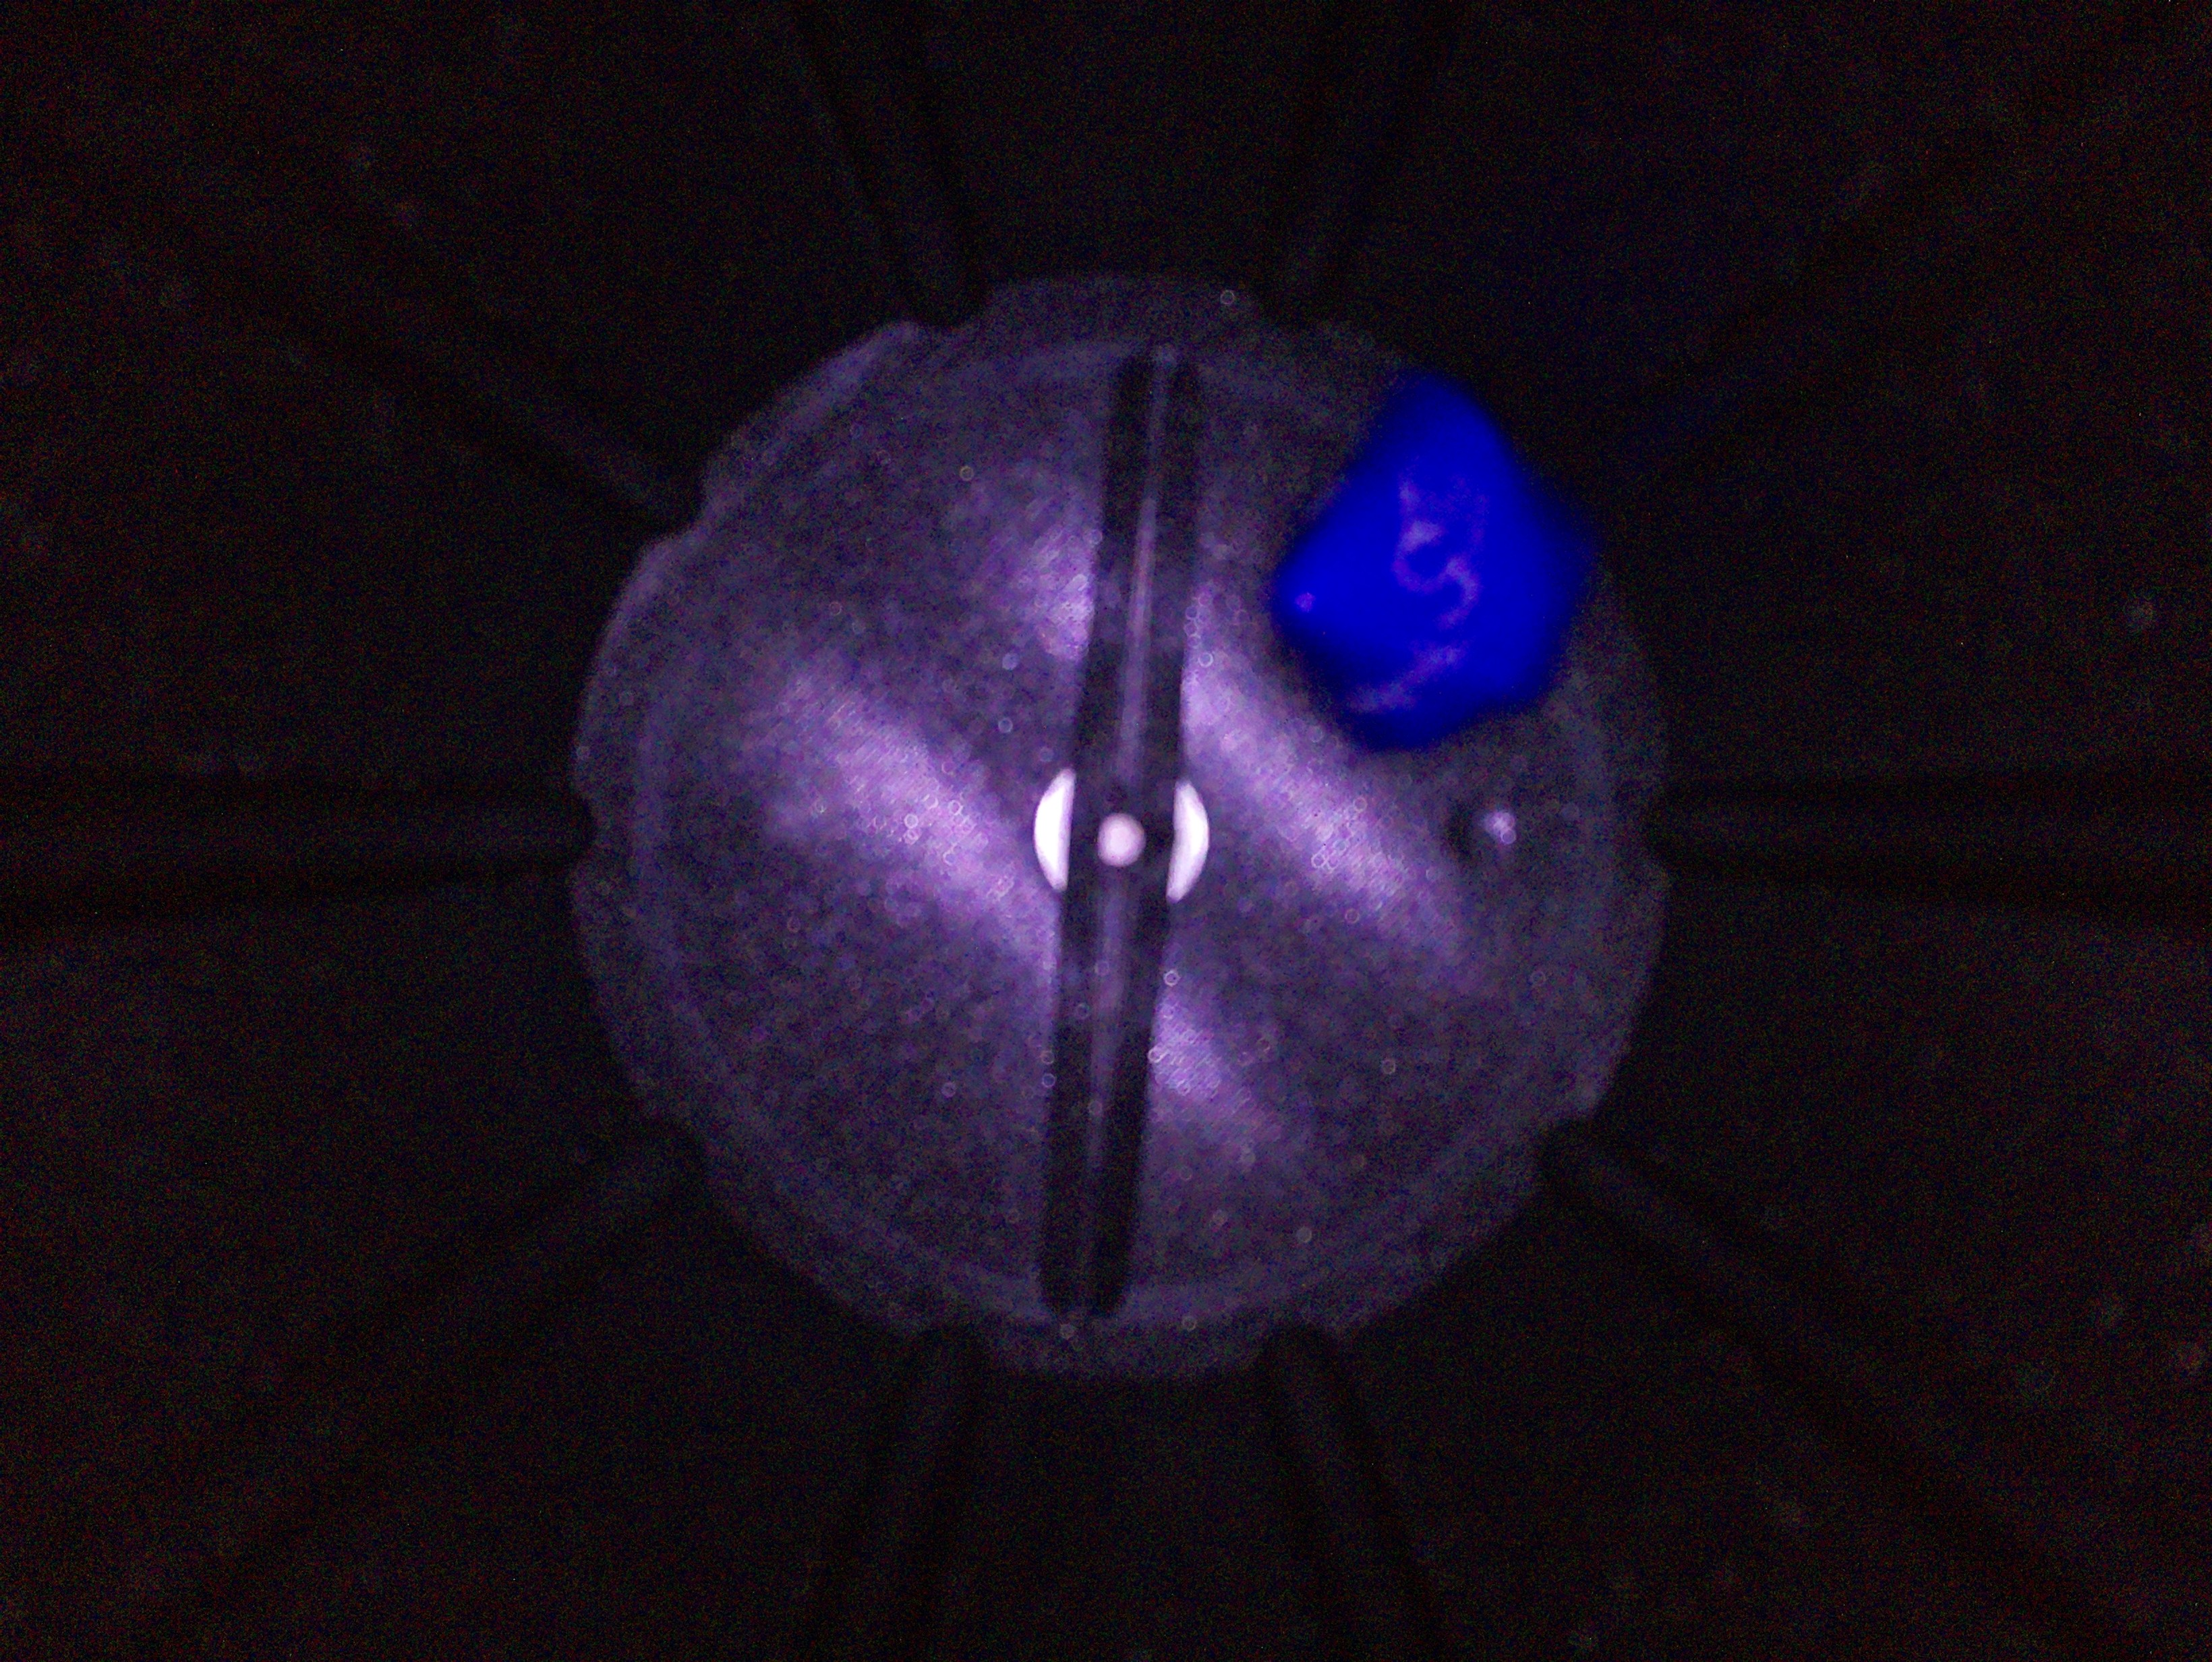
\includegraphics[width=\linewidth]{chapters/04-czytanie/figures/wir}
        \caption{Wirująca kość.}
        \label{fig:wir}
    \end{subfigure}
    \hfill
    \begin{subfigure}[t]{0.45\linewidth}
        \centering
        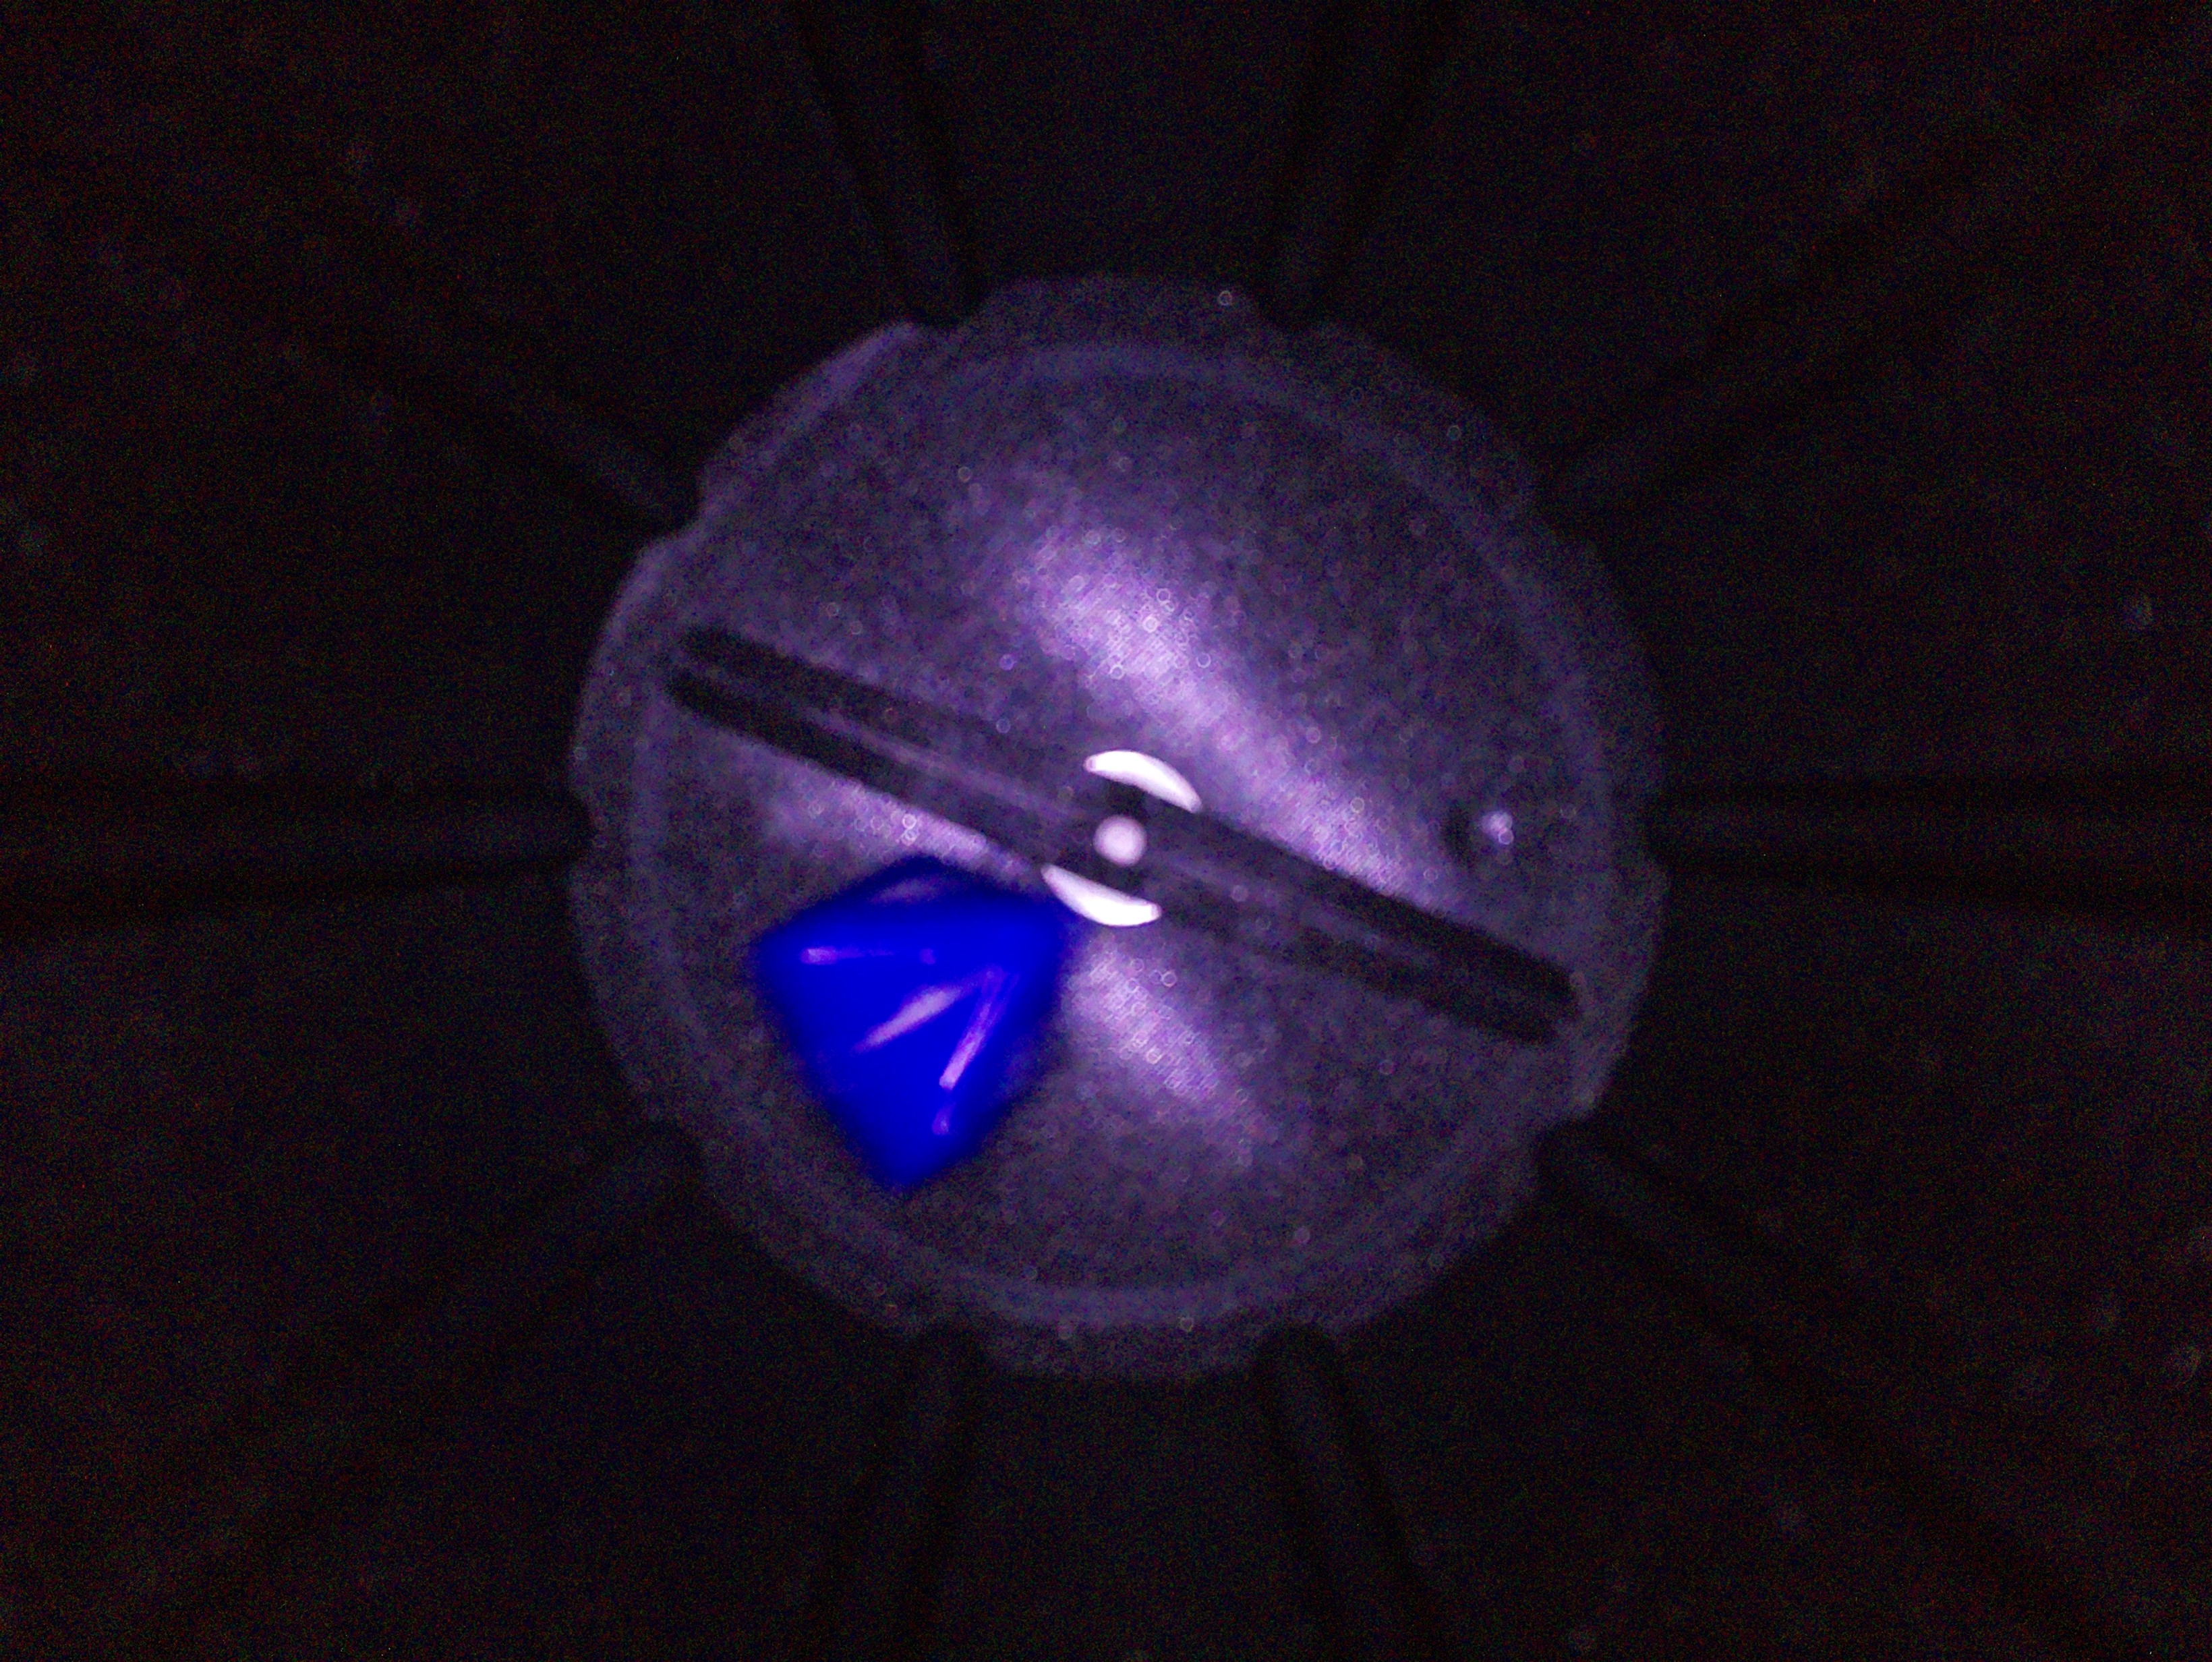
\includegraphics[width=\linewidth]{chapters/04-czytanie/figures/wir2}
        \caption{Kość w ruchu.}
        \label{fig:wir2}
    \end{subfigure}
    \caption{Nieczytelne ujęcia wynikające z dłuższego niż przewidywany ruchu kości}
    \label{fig:wircombined}
\end{figure}


Rozwiązaniem większości wypadków, w których zachodziła ta sytuacja, okazało się spowolnienie działania maszyny.
Obecnie oczekiwaniem aż kość zatrzyma się w miejscu steruje parametr czasowy, przyjmujący wartość jednej sekundy od zakończenia pracy śmigła.
Jest to wystarczające rozwiązanie, gdyż obecnie sytuacje niepewne z tego powodu zdarzają się bardzo rzadko (około 1 raz na 5000 rzutów).

Istnieje możliwość udoskonalenia tego rozwiązania, poprzez stosowanie detekcji ruchu kości,
jednak to rozwiązanie najpewniej okazałoby się bardziej kosztowne czasowo niż proste czekanie stosowane obecnie.


\subsection{Podsumowanie}\label{subsec:podsumowanie}

Przedstawiony algorytm przetwarzania wstępnego pozwala na skuteczne przygotowanie danych wejściowych dla modelu sztucznej inteligencji.
Automatyzuje proces identyfikacji i kadrowania obiektów zainteresowania w obrazach, co znacząco poprawia jakość danych.
Rozwiązanie zostało zaprojektowane z myślą o łatwej adaptacji do innych zastosowań wymagających podobnego przetwarzania obrazów,
na przykład w przypadku zmiany kości w maszynie na inną, lub z inną liczbą ścianek.

